\chapter{Iterator模式}
\section{概念}
迭代器模式(Iterator),提供一种方法顺序访问一个聚合对象中的各种元素,而又不暴露该对象的内部表示。
\par 它可以让用户透过特定的接口巡访容器中的每一个元素而不用了解底层的实现。
\par 经常要访问一个聚合对象中的各个元素,如“数据结构”中的链表遍历,通常的做法是将链表的创建和遍历都放在同一个类中,但这种方式不利于程序的扩展,如果要更换遍历方法就必须修改程序源代码,这违背了 “开闭原则”。并且有如下缺点:
\begin{itemize}
	\item 暴露了聚合类的内部表示,使其数据不安全;
	\item 增加了客户的负担。
\end{itemize}
\textbf{迭代器的优点:}
\begin{enumerate}
	\item 访问一个聚合对象的内容而无须暴露它的内部表示;
	\item 遍历任务交由迭代器完成,这简化了聚合类;
	\item 它支持以不同方式遍历一个聚合,甚至可以自定义迭代器的子类以支持新的遍历;
	\item 增加新的聚合类和迭代器类都很方便,无须修改原有代码;
	\item 封装性良好,为遍历不同的聚合结构提供一个统一的接口。
\end{enumerate}
\textbf{迭代器的缺点:}增加了类的个数,这在一定程度上增加了系统的复杂性。
\section{模式的结构}
迭代器模式是通过将聚合对象的遍历行为分离出来,抽象成迭代器类来实现的,其目的是在不暴露聚合对象的内部结构的情况下,让外部代码透明地访问聚合的内部数据。
\\ \textbf{迭代器角色:}
\begin{enumerate}
	\item 抽象聚合(Aggregate)角色:定义存储、添加、删除聚合对象以及创建迭代器对象的接口;
	\item 具体聚合(ConcreteAggregate)角色:实现抽象聚合类,返回一个具体迭代器的实例;
	\item 抽象迭代器(Iterator)角色:定义访问和遍历聚合元素的接口,通常包含 hasNext()、first()、next() 等方法;
	\item 具体迭代器(Concretelterator)角色:实现抽象迭代器接口中所定义的方法,完成对聚合对象的遍历,记录遍历的当前位置。
\end{enumerate}
\begin{figure}[!h]
	\centering
	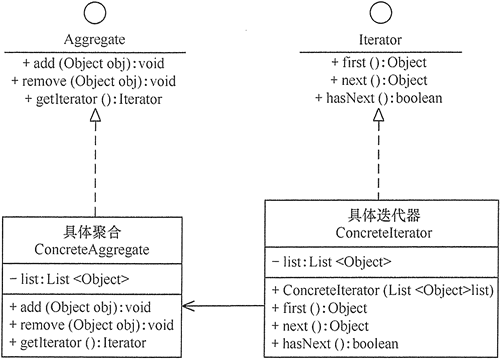
\includegraphics[width=0.8\textwidth]{image/1-1}
	\caption{迭代器模式的结构图}
\end{figure}
\section{模式的实现}
\subsection{例子一}
\begin{lstlisting}
//抽象聚合
public interface Aggregate {
	public void add(Object obj);
	public void remove(Object obj);
	public Iterator getIterator();
}
\end{lstlisting}
\begin{lstlisting}
//具体聚合
public class ConcreteAggregate implements Aggregate {
	private List<Object> list = new ArrayList<Object>();
	public void add(Object obj) {
		list.add(obj);
	}
	public void remove(Object obj) {
		list.remove(obj);
	}
	public Iterator getIterator() {
		return new ConcreteIterator(list);
	}
}
\end{lstlisting}
\begin{lstlisting}
//抽象迭代器
public interface Iterator {
	Object first();
	Object next();
	boolean hasNext();
}
\end{lstlisting}
\begin{lstlisting}
//具体迭代器
public class ConcreteIterator implements Iterator {
	private List<Object> list = null;
	private int index = -1;
	public ConcreteIterator(List<Object> list) {
		this.list = list;
	}
	public Object first() {
		index = 0;
		Object obj = list.get(index);
		return obj;
	}
	public Object next() {
		Object obj = null;
		if (this.hasNext()) {
			obj = list.get(++index);
		}
		return obj;
	}
	public boolean hasNext() {
		if (index < list.size() - 1) {
			return true;
		} else {
			return false;
		}
	}
}
\end{lstlisting}
\begin{lstlisting}
public class IteratorPattern {
	public static void main(String[] args) {
		Aggregate ag = new ConcreteAggregate();
		ag.add("item 1");
		ag.add("Item 2");
		ag.add(6);
		ag.add(6.7);
		Iterator it = ag.getIterator();
		while (it.hasNext()) {
			Object o = it.next();
			System.out.print(o.toString() + " ");
		}
	}
}
\end{lstlisting}
\subsection{例子二}
\begin{lstlisting}
//Aggregate表示集合的接口
public interface Aggregate {
	public abstract Iterator iterator();
}
\end{lstlisting}
\begin{lstlisting}
//Iterator遍历集合的接口
public interface Iterator {
	public abstract boolean hasNext();
	public abstract Object next();
}
\end{lstlisting}
\begin{lstlisting}
//Book表示书的类
public class Book {
	private String name;
	public Book(String n){
		name = n;
	}
	public String getName() {
		return name;
	}
	public void setName(String name) {
		this.name = name;
	}
}
\end{lstlisting}
\begin{lstlisting}
//BookShelf表示书架的类
public class BookShelf implements Aggregate{
	private Book[] books;
	private int last = 0;
	public BookShelf(int maxsize) {
		this.books = new Book[maxsize];
	}
	public Book getBookAt(int index) {
		return books[index];
	}
	public void appendBook(Book book) {
		this.books[last] = book;
		last++;
	}
	public int getLength() {
		return last;
	}
	public Iterator iterator() {
		return new BookShelfIterator(this);
	}
}
\end{lstlisting}
\begin{lstlisting}
//BookShelfIterator遍历书架的类
public class BookShelfIterator implements Iterator {
	private BookShelf bookShelf;
	private int index;
	public BookShelfIterator(BookShelf bookShelf) {
		this.bookShelf = bookShelf;
		this.index = 0;
	}
	public boolean hasNext() {
		if (index < bookShelf.getLength()) {
			return true;
		} else {
			return false;
		}
	}
	public Object next() {
		Book book = bookShelf.getBookAt(index);
		index++;
		return book;
	}
}
\end{lstlisting}
\begin{lstlisting}
//Main测试程序行为的类
public class Main {
	public static void main(String[] args) {
		BookShelf bookShelf = new BookShelf(4);
		bookShelf.appendBook(new Book("天气"));
		bookShelf.appendBook(new Book("浮士德"));
		bookShelf.appendBook(new Book("Fool"));
		bookShelf.appendBook(new Book("常守朱"));
		Iterator it = bookShelf.iterator();
		while (it.hasNext()) {
			Book book = (Book) it.next();
			System.out.println(book.getName());
		}
	}
}
\end{lstlisting}
\subsection{Iterator解析}
\noindent \textbf{Iterator}
\par 负责定义按顺序遍历元素的接口API。
\\ \textbf{ConcreteIterator}
\par 负责实现Iterator角色中所定义的API。
\\ \textbf{Aggregate}
\par 负责定义创建Iterator角色的接口API。
\\ \textbf{ConcreteAggregate}
\par 负责实现Aggregate角色中所定义的接口API。
\subsection{拓展思路}
\subsubsection{不管如何变化,都可以使用Iterator}
在书架例子中,引入Iterator将遍历和实现分离开,使得遍历并没有调用
BookShelf中的方法,while不依赖于BookShelf的实现,因此这对于BookShelf的改变也能适应,
如:在BookShelf中Book[]改为ArrayList
\subsubsection{难以理解抽象类和接口}
不建议使用具体类编程,可以使用抽象类作为接口编程,否则会导致类之间强耦合。
\subsubsection{Aggregate和Iterator}
虽然while不依赖于BookShelf,但是对于BookShelfIterator要知道BookShelf是如何实现的,
因此如果BookShelf发生变化,必须修改BookShelfIterator。
\subsubsection{注意}
\begin{itemize}
	\item next是“返回当前元素,并指向下一个元素”;
	\item hasNext“确认接下来是否可以调用next方法”;
	\item 一个聚合类可以有多个Iterator;
	\item 迭代器遍历方式:
	\subitem 从最后向前;
	\subitem 可前可后遍历;
	\subitem 跳跃式遍历;
	\item 这里使用的是new一个Iterator作为Main中引用目标,而不是封装在具体聚合类中,
	因此,只要Main中it=null,GC会自动回收。
\end{itemize}